\section{MODEL: AUGMENTED GRAPH SLAM}
\label{sec:model}
%\begin{wrapfigure}{r}{0.25\textwidth}
\begin{figure}[!t]
\begin{center}
%\framebox[4.0in]{$\;$}
%\fbox{\rule[-.5cm]{0cm}{4cm} \rule[-.5cm]{4cm}{0cm}}
 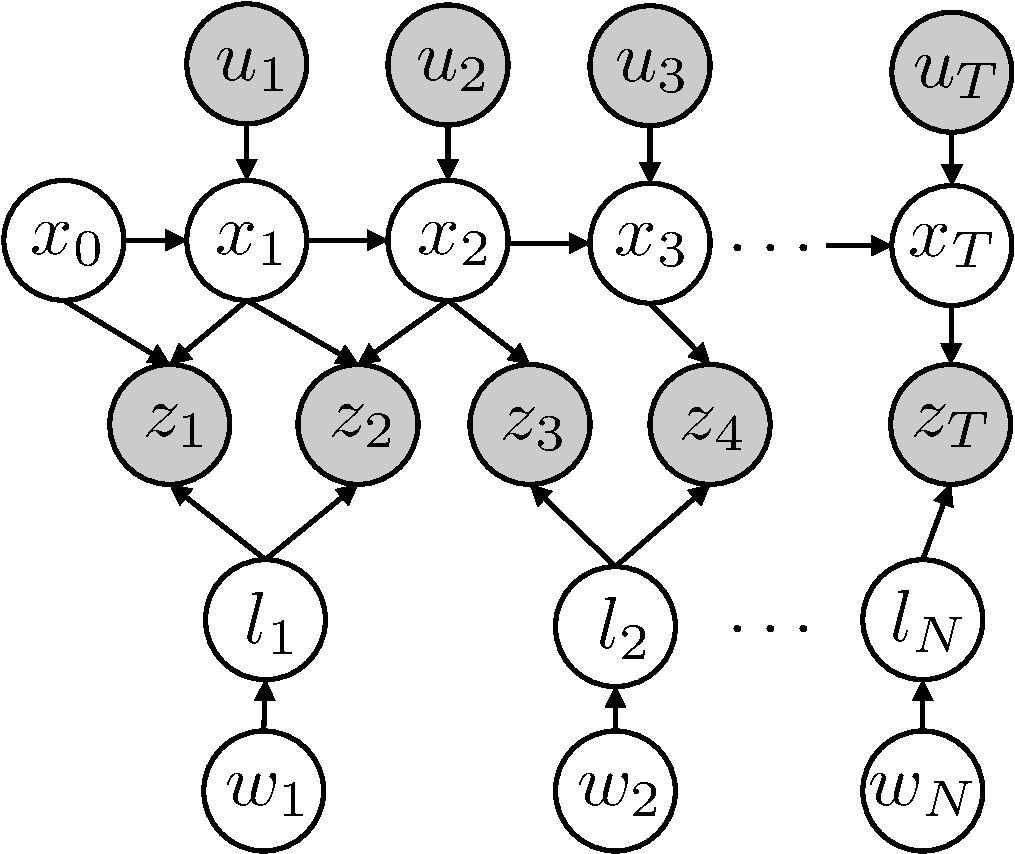
\includegraphics[width=0.5\columnwidth]{fig/model} 
\end{center}
\caption{Graphical Model Formulation. Dark nodes are observed.}
\label{fig:model}
\end{figure}
%\end{wrapfigure}

Following \cite{isam} we formulate the SLAM problem in graphical models as in Figure \ref{fig:model}. Specifically, the robot states (as position and orientation over time in map coordinates) are denoted by $X = \{\boldsymbol{x}_i\}$ with $i \in 0, \dots T$, the landmark locations in map coordinates by $L = \{\boldsymbol{l}_j\}$ with $j \in 1,\dots, N$, the control inputs for movement by $U = \{\boldsymbol{u}_i\}$ for $i \in 1,\dots, T$ and the landmark measurements in robot coordinates by $Z = \{\boldsymbol{z}_k\}$ with $k \in 1, \dots, K$. In addition to the classical graph SLAM formulation, we augment the representation of landmarks with a set of $N$ scalar latent parameters $W = \{w_j\}$ with $j \in 1, \dots, N$. At each time $k$, the measurement $\boldsymbol{z}_k$ corresponds to robot pose $\boldsymbol{x}_{i_k}$, landmark $\boldsymbol{l}_{j_k}$, and latent variable $w_{j_k}$, where $i_k$ associates robot poses with measurements, and $j_k$ associates landmarks with measurements.

%resolved \cj{is W for data associateion? if so, this should be stated explicitly xlz: how about this? cjenkins: better, i added a little more}

In considering dynamic environments, $W$ models the mobility of each landmark about whether it is capable of movement or not without considering extra kinematics, and robustify the observation term of the model in Equation \ref{eq:sensor}.  Through $W$, corrupted measurements associated with moving landmarks are suitably eliminated as outliers from the mapping process. It may be appealing to model a dynamically moving object as a sequence of variables. However, it is shown in the following that the scalar mobility variables are adequate enough to eliminate moving landmarks from graph optimization.

According to the proposed graphical model, we give the joint probability of all variables and measurements as:
%\begin{equation}
\begin{multline}
P(X, L, U, Z, W) \propto  \\
\prod\limits_{i}P(\boldsymbol{x}_i|\boldsymbol{x}_{i-1}, \boldsymbol{u}_i)\prod\limits_{k}P(\boldsymbol{z}_k|\boldsymbol{x}_{i_k}, \boldsymbol{l}_{j_k}, w_{j_k}).
\label{eq:jointProb}
\end{multline}
%\end{equation}

Then the maximum likelihood (ML) estimate of the unobserved poses $X$ and landmarks $L$ given observations $Z$, known controls $U$, and the current latent parameters $W$ are defined as

\begin{equation}
X^*, L^* = \operatorname*{arg\,max}_{X,L} P(X,L,U,Z,W).
\end{equation}

To calculate the ML estimate, the objective is linearized and converted into a linear least
squares problem in this form $\operatorname*{arg\,min}_{\boldsymbol{\delta}} || \boldsymbol{A}
\boldsymbol{\delta}  - \boldsymbol{b} ||^2$ by algebraic manipulation, and then optimized using
different numerical methods. Derivation with more details is provided in appendix \ref{appendix:leastsquare}.

Using a Gaussian representation with the latent extension, the sensor
model, the process model and measurement equation are defined as

\begin{equation}
\begin{aligned}
\boldsymbol{x}_i &= f_i(\boldsymbol{x}_{i-1}, \boldsymbol{u}_i) + \boldsymbol{\eta}_i \\
\boldsymbol{z}_k &= h_k(\boldsymbol{x}_{i_k}, \boldsymbol{l}_{j_k}) + \boldsymbol{\theta}_k
\end{aligned}
\label{eq:gaussRepresentation}
\end{equation}

where $\boldsymbol{\eta}_i$ and $\boldsymbol{\theta}_k$ are noise terms which follow zero-mean Gaussian distribution with covariance matrices $\boldsymbol{\Gamma}_i$ and $\boldsymbol{\Sigma}_k$. With this formulation, the second part of the joint probability \ref{eq:jointProb} is augmented with the mobility indicator. In addition we also apply a robust kernel $v_k$ to the observation term, then the conditional probability of $\boldsymbol{z}_k$ is defined as an augmented Gaussian distribution:

%resolved \cj{need to reformat exp() to be within margin, e is placeholder, xlz: fixed, cjenkins: added aligned}
\begin{equation}
\begin{aligned}
P(\boldsymbol{z}_k|\boldsymbol{x}_{i_k}, \boldsymbol{l}_{j_k}, w_{j_k})\propto \exp(-w_{j_k} \tilde{\boldsymbol{\mu}}_k^T \boldsymbol{\Sigma}_k^{-1} \tilde{\boldsymbol{\mu}}_k),\\
 \tilde{\boldsymbol{\mu}}_k = v_k(h_k(\boldsymbol{x}_{i_k}, \boldsymbol{l}_{j_k}) - \boldsymbol{z}_k)
 %e^{(-w_{j_k} (v_k(z_k - h_k(x_{i_k}, l_{j_k})))^T \Sigma_k^{-1} (v_k(z_k - h_k(x_{i_k}, l_{j_k}))) }.
 %\exp(-w_{j_k} (v_k(z_k - h_k(x_{i_k}, l_{j_k})))^T \Sigma_k^{-1} (v_k(z_k - h_k(x_{i_k}, l_{j_k}))) ).
\label{eq:sensor}
\end{aligned}
\end{equation}

where $w_{j_k}$ represents the likelihood of being static for landmark $\boldsymbol{l}_{j_k}$ associated with measurement $\boldsymbol{z}_k$ at time $k$, and $v_k$ is the robust scaling factor associated with each landmark observation representing whether the measurement is an inlier. When $w_{j_k}$ or $v_k$ approaches zero, the effect is equivalent to making the covariance of the Gaussian very large, effectively rendering the distribution uniform and the constraint represented by the distribution of no impact on the graph optimization process. Note that $w_{j_k}$ can be negative because the formulation given here is proportional to a normalizing constant.
% In our case, we need to infer what their values are and ideally whether the process could be online or folows an incremental fashion. Possible solutions could be 1) using visual cues to cluster the landmarks to ``moving''/``static''. Challenges mainly lies in whether the features we use is reliable or not in terms of this clustering task; 2) instead of using an expensive EM algorithm in \cite{rogers2010slam}, we design particle filters to incrementally update parameter $w_k$, making the whole process online.
